\documentclass[a4paper]{article}

\usepackage[english]{babel}
\usepackage{tikz,pgf}
\usetikzlibrary{arrows,automata}
\usepackage{verbatim}
\usepackage[fleqn,tbtags]{mathtools}
\usepackage{tikz,fullpage}
\usepackage{tkz-berge}
\usepackage{adjustbox}
\usepackage{subfig}
\usepackage[hidelinks]{hyperref}
\usepackage{color}

\newcommand{\subject}{Automata Theory and Formal Language}
\newcommand{\practice}{Lab Session 4}

\title{\subject \\ \practice}
\author{{\large Carlos Gallardo Polanco } \\ {\small  mail@mail.com
}
             \\ {\small \url{https://github.com/gpcarlos95/TALFPractice}}}
\date{\today}


\newcommand{\ENFA}{{\Large $\varepsilon$}$-NFA$ }

\begin{document}
\maketitle
\newpage

\section{Exercise}
  Given the $RE$ $E=(((00)*+(00)*0)10 + ((11)*+(11)*1)10)*$
  \begin{enumerate}
    \item Build a \ENFA thats accepts exactly the same
          language, following the method explained in class to convert from
          $RE$ to \ENFA.
    \item Generate the equivalent $DFA$
    \item Implement it in a programming language (\verb!Python!,
          \verb!C!/\verb!C++!, \verb!Java!) following the table method.
  \end{enumerate} 

\section{Solution}
  \begin{enumerate}
    \item Build a \ENFA thats accepts exactly the same
          language, following the method explained in class to convert from
          $RE$ to \ENFA. \\ \\
          To convert a $ER$ to an \ENFA we'll follow the following equivalences:
\begin{itemize}
  \item Union. \\
        If $E1=0$ and $E2=0$ then $E1 \cup E2$ ($E1+E2$): \\ \\

        \begin{center}
        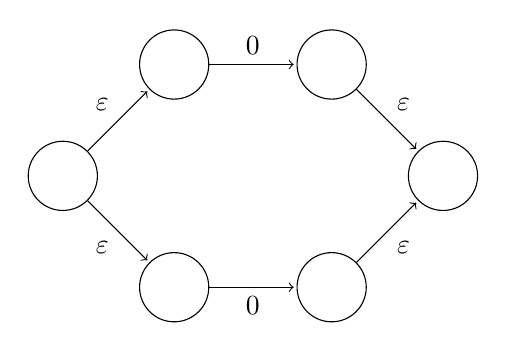
\begin{tikzpicture}[shorten >=1pt,node distance=2cm,auto]

          \node[state]  (A)                     { };
          \node[state]  (B) [above right of=A]  { };
          \node[state]  (C) [right of=B]        { };
          \node[state]  (D) [below right of=A]  { };
          \node[state]  (E) [right of=D]        { };
          \node[state]  (F) [above right of=E]  { };

          \path[->] (A) edge node         {$\varepsilon$} (B)
                        edge node [swap]  {$\varepsilon$} (D)
                    (B) edge node         {0}             (C)
                    (C) edge node         {$\varepsilon$} (F)
                    (D) edge node [swap]  {0} (E)
                    (E) edge node [swap]  {$\varepsilon$} (F);
        \end{tikzpicture}
        \end{center}


  \item Concatenation. \\
        If $E1=0$ and $E2=0$ then $E1E2$: \\ \\

        \begin{center}
        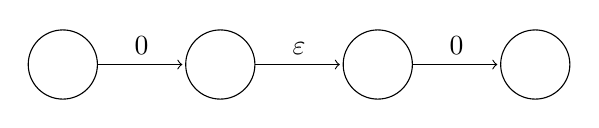
\begin{tikzpicture}[shorten >=1pt,node distance=2cm,auto]

          \node[state]  (A)               { };
          \node[state]  (B) [right of=A]  { };
          \node[state]  (C) [right of=B]  { };
          \node[state]  (D) [right of=C]  { };

          \path[->] (A) edge node         {0} (B)
                    (B) edge node         {$\varepsilon$} (C)
                    (C) edge node         {0} (D);
        \end{tikzpicture}
        \end{center}

  \item Concatenation. \\
        If $E=0$ then $E*$: \\

        \begin{center}
        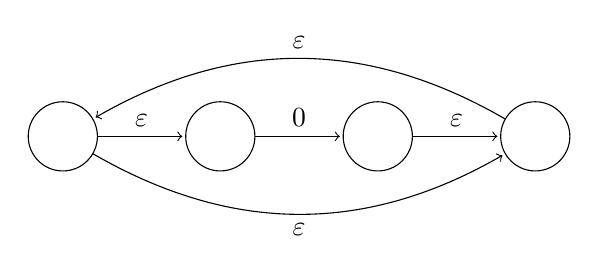
\begin{tikzpicture}[shorten >=1pt,node distance=2cm,auto]

          \node[state]  (A)               { };
          \node[state]  (B) [right of=A]  { };
          \node[state]  (C) [right of=B]  { };
          \node[state]  (D) [right of=C]  { };

          \path[->] (A) edge node                     {$\varepsilon$} (B)
                        edge [bend right] node [swap] {$\varepsilon$} (D)
                    (B) edge node                     {0}             (C)
                    (C) edge node                     {$\varepsilon$} (D)
                    (D) edge [bend right] node [swap] {$\varepsilon$} (A);
        \end{tikzpicture}
        \end{center}

\end{itemize}

\newpage
We'll divide the main $ER$ into smaller $ER$s:

    $$E=\underbracket{(\underbracket{(\underbracket{(\underbracket{\underbracket{
    \underbracket{(00)}_{E1}*}_{E1*}+\underbracket{\underbracket{
    \underbracket{(00)}_{E1}*}_{E1*}0}_{E3}}_{E5})10}_{E7} +
    \underbracket{(\underbracket{\underbracket{\underbracket{(11)}_{E2}*}_{E2*}+
    \underbracket{\underbracket{
    \underbracket{(11)}_{E2}*}_{E2*}1}
    _{E4}}_{E6})10}_{E8})}_{E9}*}_{E9*=E}$$

    \begin{itemize}
      \item $E1=00$ \\
      \begin{center}
      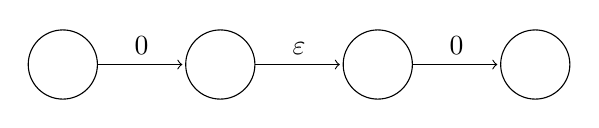
\begin{tikzpicture}[shorten >=1pt,node distance=2cm,auto]

        \node[state]  (Q01)                 { };
        \node[state]  (Q02) [right of=Q01]  { };
        \node[state]  (Q03) [right of=Q02]  { };
        \node[state]  (Q04) [right of=Q03]  { };

        \path[->] (Q01) edge node                     {0}             (Q02)
                  (Q02) edge node                     {$\varepsilon$} (Q03)
                  (Q03) edge node                     {0}             (Q04);
      \end{tikzpicture}
      \end{center}

      \item $E1*=(00)*$ \\
      \begin{center}
      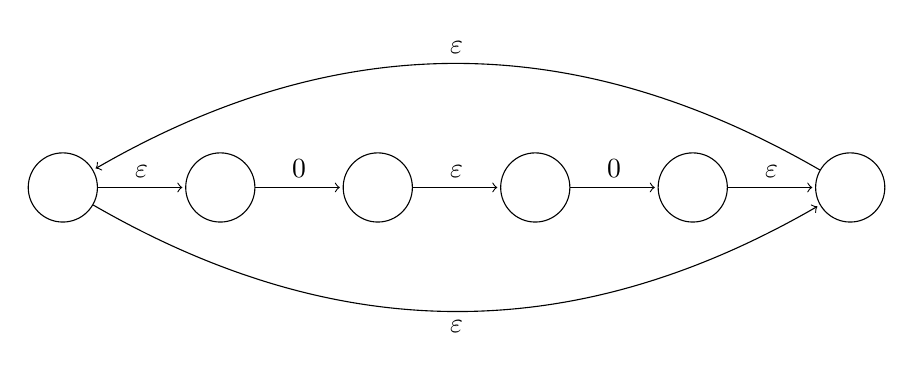
\begin{tikzpicture}[shorten >=1pt,node distance=2cm,auto]

        \node[state]  (Q01)                 { };
        \node[state]  (Q02) [right of=Q01]  { };
        \node[state]  (Q03) [right of=Q02]  { };
        \node[state]  (Q04) [right of=Q03]  { };
        \node[state]  (Q05) [right of=Q04]  { };
        \node[state]  (Q06) [right of=Q05]  { };

        \path[->]
                  (Q01) edge node                     {$\varepsilon$} (Q02)
                        edge [bend right] node [swap] {$\varepsilon$} (Q06)
                  (Q02) edge node                     {0}             (Q03)
                  (Q03) edge node                     {$\varepsilon$} (Q04)
                  (Q04) edge node                     {0}             (Q05)
                  (Q05) edge node                     {$\varepsilon$} (Q06)
                  (Q06) edge [bend right] node [swap] {$\varepsilon$} (Q01);
      \end{tikzpicture}
      \end{center}

      \item $E2=11$ \\
      \begin{center}
      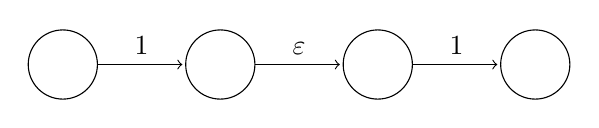
\begin{tikzpicture}[shorten >=1pt,node distance=2cm,auto]

        \node[state]  (Q01)                 { };
        \node[state]  (Q02) [right of=Q01]  { };
        \node[state]  (Q03) [right of=Q02]  { };
        \node[state]  (Q04) [right of=Q03]  { };

        \path[->] (Q01) edge node                     {1}             (Q02)
                  (Q02) edge node                     {$\varepsilon$} (Q03)
                  (Q03) edge node                     {1}             (Q04);
      \end{tikzpicture}
      \end{center}

      \item $E2*=(11)*$ \\
      \begin{center}
      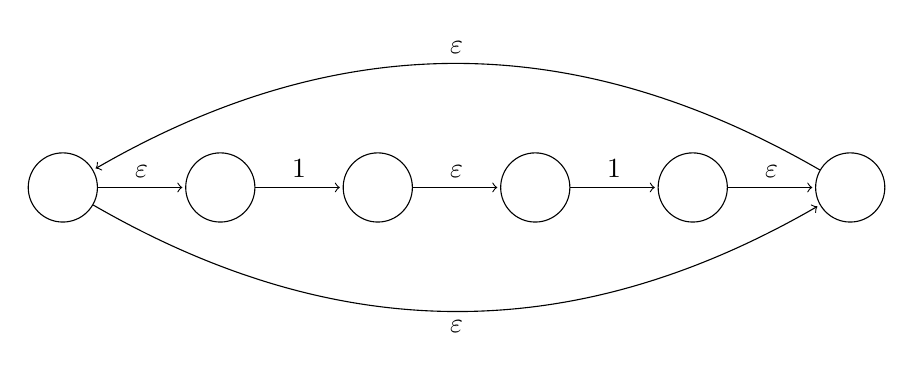
\begin{tikzpicture}[shorten >=1pt,node distance=2cm,auto]

        \node[state]  (Q01)                 { };
        \node[state]  (Q02) [right of=Q01]  { };
        \node[state]  (Q03) [right of=Q02]  { };
        \node[state]  (Q04) [right of=Q03]  { };
        \node[state]  (Q05) [right of=Q04]  { };
        \node[state]  (Q06) [right of=Q05]  { };

        \path[->]
                  (Q01) edge node                     {$\varepsilon$} (Q02)
                        edge [bend right] node [swap] {$\varepsilon$} (Q06)
                  (Q02) edge node                     {1}             (Q03)
                  (Q03) edge node                     {$\varepsilon$} (Q04)
                  (Q04) edge node                     {1}             (Q05)
                  (Q05) edge node                     {$\varepsilon$} (Q06)
                  (Q06) edge [bend right] node [swap] {$\varepsilon$} (Q01);
      \end{tikzpicture}
      \end{center}
\newpage
      \item $E3=(00)*0$ \\
      \begin{center}
      \begin{adjustbox}{max width=13cm}
      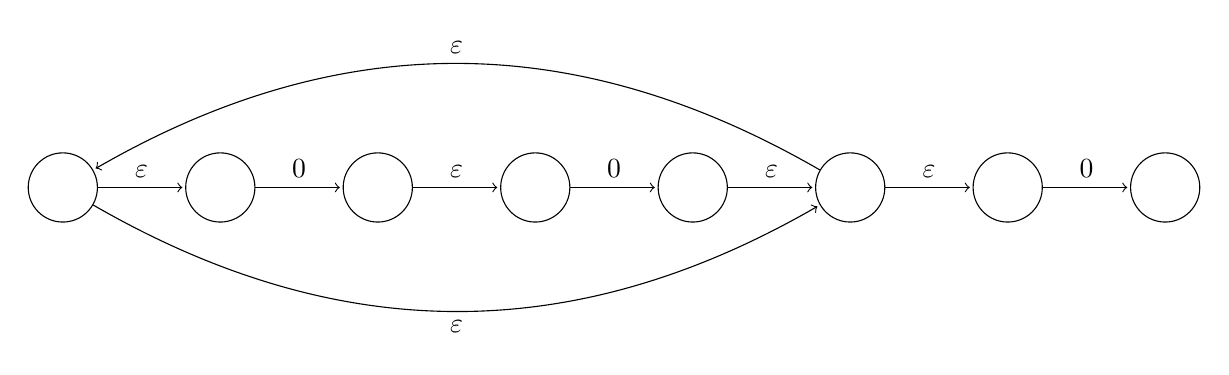
\begin{tikzpicture}[shorten >=1pt,node distance=2cm,auto]

        \node[state]  (Q01)                 { };
        \node[state]  (Q02) [right of=Q01]  { };
        \node[state]  (Q03) [right of=Q02]  { };
        \node[state]  (Q04) [right of=Q03]  { };
        \node[state]  (Q05) [right of=Q04]  { };
        \node[state]  (Q06) [right of=Q05]  { };
        \node[state]  (Q07) [right of=Q06]  { };
        \node[state]  (Q08) [right of=Q07]  { };

        \path[->]
                  (Q01) edge node                     {$\varepsilon$} (Q02)
                        edge [bend right] node [swap] {$\varepsilon$} (Q06)
                  (Q02) edge node                     {0}             (Q03)
                  (Q03) edge node                     {$\varepsilon$} (Q04)
                  (Q04) edge node                     {0}             (Q05)
                  (Q05) edge node                     {$\varepsilon$} (Q06)
                  (Q06) edge [bend right] node [swap] {$\varepsilon$} (Q01)
                        edge node                     {$\varepsilon$} (Q07)
                  (Q07) edge node                     {0}             (Q08);
      \end{tikzpicture}
      \end{adjustbox}
      \end{center}

      \item $E4=(11)*1$ \\
      \begin{center}
      \begin{adjustbox}{max width=13cm}
      \begin{tikzpicture}[shorten >=1pt,node distance=2cm,auto]

        \node[state]  (Q01)                 { };
        \node[state]  (Q02) [right of=Q01]  { };
        \node[state]  (Q03) [right of=Q02]  { };
        \node[state]  (Q04) [right of=Q03]  { };
        \node[state]  (Q05) [right of=Q04]  { };
        \node[state]  (Q06) [right of=Q05]  { };
        \node[state]  (Q07) [right of=Q06]  { };
        \node[state]  (Q08) [right of=Q07]  { };

        \path[->]
                  (Q01) edge node                     {$\varepsilon$} (Q02)
                        edge [bend right] node [swap] {$\varepsilon$} (Q06)
                  (Q02) edge node                     {1}             (Q03)
                  (Q03) edge node                     {$\varepsilon$} (Q04)
                  (Q04) edge node                     {1}             (Q05)
                  (Q05) edge node                     {$\varepsilon$} (Q06)
                  (Q06) edge [bend right] node [swap] {$\varepsilon$} (Q01)
                        edge node                     {$\varepsilon$} (Q07)
                  (Q07) edge node                     {1}             (Q08);
      \end{tikzpicture}
      \end{adjustbox}
      \end{center}

      \item $E5=(00)*+(00)*0$ \\
      \begin{center}
      \begin{adjustbox}{max width=13cm}
      \begin{tikzpicture}[shorten >=1pt,node distance=2cm,auto]
        \tikzstyle{invisible}=[draw=white]

        \node[state,invisible]  (I01)             { };
        \node[state]  (Q09) [above of=I01]        { }; % E2*
        \node[state]  (Q10) [right of=Q09]        { };
        \node[state]  (Q11) [right of=Q10]        { };
        \node[state]  (Q12) [right of=Q11]        { };
        \node[state]  (Q13) [right of=Q12]        { };
        \node[state]  (Q14) [right of=Q13]        { };
        \node[state]  (Q01) [below of=I01]        { }; % E4
        \node[state]  (Q02) [right of=Q01]        { };
        \node[state]  (Q03) [right of=Q02]        { };
        \node[state]  (Q04) [right of=Q03]        { };
        \node[state]  (Q05) [right of=Q04]        { };
        \node[state]  (Q06) [right of=Q05]        { };
        \node[state]  (Q07) [right of=Q06]        { };
        \node[state]  (Q08) [right of=Q07]        { };
        \node[state]  (Q15) [left of=I01]         { };
        \node[state,invisible]  (I02) [above of=Q08] { };
        \node[state]  (Q16) [right of=I02]        { };

        \path[->]
                  (Q09) edge node                     {$\varepsilon$} (Q10)% E2*
                        edge [bend right] node [swap] {$\varepsilon$} (Q14)
                  (Q10) edge node                     {0}             (Q11)
                  (Q11) edge node                     {$\varepsilon$} (Q12)
                  (Q12) edge node                     {0}             (Q13)
                  (Q13) edge node                     {$\varepsilon$} (Q14)
                  (Q14) edge [bend right] node [swap] {$\varepsilon$} (Q09)
                  (Q14) edge node                     {$\varepsilon$} (Q16)
                  (Q01) edge node                     {$\varepsilon$} (Q02)% E4
                        edge [bend right] node [swap] {$\varepsilon$} (Q06)
                  (Q02) edge node                     {0}             (Q03)
                  (Q03) edge node                     {$\varepsilon$} (Q04)
                  (Q04) edge node                     {0}             (Q05)
                  (Q05) edge node                     {$\varepsilon$} (Q06)
                  (Q06) edge [bend right] node [swap] {$\varepsilon$} (Q01)
                        edge node                     {$\varepsilon$} (Q07)
                  (Q07) edge node                     {0}             (Q08)
                  (Q08) edge node [swap]              {$\varepsilon$} (Q16)
                  (Q15) edge node                     {$\varepsilon$} (Q09)
                        edge node [swap]              {$\varepsilon$} (Q01);
      \end{tikzpicture}
      \end{adjustbox}
      \end{center}

      \item $E6=(11)*+(11)*1$ \\
      \begin{center}
      \begin{adjustbox}{max width=13cm}
      \begin{tikzpicture}[shorten >=1pt,node distance=2cm,auto]
        \tikzstyle{invisible}=[draw=white]

        \node[state,invisible]  (I01)             { };
        \node[state]  (Q09) [above of=I01]        { }; % E2*
        \node[state]  (Q10) [right of=Q09]        { };
        \node[state]  (Q11) [right of=Q10]        { };
        \node[state]  (Q12) [right of=Q11]        { };
        \node[state]  (Q13) [right of=Q12]        { };
        \node[state]  (Q14) [right of=Q13]        { };
        \node[state]  (Q01) [below of=I01]        { }; % E4
        \node[state]  (Q02) [right of=Q01]        { };
        \node[state]  (Q03) [right of=Q02]        { };
        \node[state]  (Q04) [right of=Q03]        { };
        \node[state]  (Q05) [right of=Q04]        { };
        \node[state]  (Q06) [right of=Q05]        { };
        \node[state]  (Q07) [right of=Q06]        { };
        \node[state]  (Q08) [right of=Q07]        { };
        \node[state]  (Q15) [left of=I01]         { };
        \node[state,invisible]  (I02) [above of=Q08] { };
        \node[state]  (Q16) [right of=I02]        { };

        \path[->]
                  (Q09) edge node                     {$\varepsilon$} (Q10)% E2*
                        edge [bend right] node [swap] {$\varepsilon$} (Q14)
                  (Q10) edge node                     {1}             (Q11)
                  (Q11) edge node                     {$\varepsilon$} (Q12)
                  (Q12) edge node                     {1}             (Q13)
                  (Q13) edge node                     {$\varepsilon$} (Q14)
                  (Q14) edge [bend right] node [swap] {$\varepsilon$} (Q09)
                  (Q14) edge node                     {$\varepsilon$} (Q16)
                  (Q01) edge node                     {$\varepsilon$} (Q02)% E4
                        edge [bend right] node [swap] {$\varepsilon$} (Q06)
                  (Q02) edge node                     {1}             (Q03)
                  (Q03) edge node                     {$\varepsilon$} (Q04)
                  (Q04) edge node                     {1}             (Q05)
                  (Q05) edge node                     {$\varepsilon$} (Q06)
                  (Q06) edge [bend right] node [swap] {$\varepsilon$} (Q01)
                        edge node                     {$\varepsilon$} (Q07)
                  (Q07) edge node                     {1}             (Q08)
                  (Q08) edge node [swap]              {$\varepsilon$} (Q16)
                  (Q15) edge node                     {$\varepsilon$} (Q09)
                        edge node [swap]              {$\varepsilon$} (Q01);
      \end{tikzpicture}
      \end{adjustbox}
      \end{center}

      \item $E7=((00)*+(00)*0)10$ \\
      \begin{center}
      \begin{adjustbox}{max width=13cm}
      \begin{tikzpicture}[shorten >=1pt,node distance=2cm,auto]
        \tikzstyle{invisible}=[draw=white]

        \node[state,invisible]  (I01)             { };
        \node[state]  (Q15) [left of=I01]         { };
        \node[state]  (Q09) [above of=I01]        { }; % E1*
        \node[state]  (Q10) [right of=Q09]        { };
        \node[state]  (Q11) [right of=Q10]        { };
        \node[state]  (Q12) [right of=Q11]        { };
        \node[state]  (Q13) [right of=Q12]        { };
        \node[state]  (Q14) [right of=Q13]        { };
        \node[state]  (Q01) [below of=I01]        { }; % E3
        \node[state]  (Q02) [right of=Q01]        { };
        \node[state]  (Q03) [right of=Q02]        { };
        \node[state]  (Q04) [right of=Q03]        { };
        \node[state]  (Q05) [right of=Q04]        { };
        \node[state]  (Q06) [right of=Q05]        { };
        \node[state]  (Q07) [right of=Q06]        { };
        \node[state]  (Q08) [right of=Q07]        { };
        \node[state,invisible]  (I02) [above of=Q08] { };
        \node[state]  (Q16) [right of=I02]        { };
        \node[state]  (Q17) [right of=Q16]        { };
        \node[state]  (Q18) [right of=Q17]        { };
        \node[state]  (Q19) [right of=Q18]        { };
        \node[state]  (Q20) [right of=Q19]        { };

        \path[->]
                  (Q09) edge node                     {$\varepsilon$} (Q10)% E1*
                        edge [bend right] node [swap] {$\varepsilon$} (Q14)
                  (Q10) edge node                     {0}             (Q11)
                  (Q11) edge node                     {$\varepsilon$} (Q12)
                  (Q12) edge node                     {0}             (Q13)
                  (Q13) edge node                     {$\varepsilon$} (Q14)
                  (Q14) edge [bend right] node [swap] {$\varepsilon$} (Q09)
                  (Q14) edge node                     {$\varepsilon$} (Q16)
                  (Q01) edge node                     {$\varepsilon$} (Q02)% E3
                        edge [bend right] node [swap] {$\varepsilon$} (Q06)
                  (Q02) edge node                     {0}             (Q03)
                  (Q03) edge node                     {$\varepsilon$} (Q04)
                  (Q04) edge node                     {0}             (Q05)
                  (Q05) edge node                     {$\varepsilon$} (Q06)
                  (Q06) edge [bend right] node [swap] {$\varepsilon$} (Q01)
                        edge node                     {$\varepsilon$} (Q07)
                  (Q07) edge node                     {0}             (Q08)
                  (Q08) edge node [swap]              {$\varepsilon$} (Q16)
                  (Q15) edge node                     {$\varepsilon$} (Q09)
                        edge node [swap]              {$\varepsilon$} (Q01)
                  (Q16) edge node                     {$\varepsilon$} (Q17)
                  (Q17) edge node                     {1}             (Q18)
                  (Q18) edge node                     {$\varepsilon$} (Q19)
                  (Q19) edge node                     {0}             (Q20);
      \end{tikzpicture}
      \end{adjustbox}
      \end{center}

      \item $E8=((11)*+(11)*1)10$ \\
      \begin{center}
      \begin{adjustbox}{max width=13cm}
      \begin{tikzpicture}[shorten >=1pt,node distance=2cm,auto]
        \tikzstyle{invisible}=[draw=white]

        \node[state,invisible]  (I01)             { };
        \node[state]  (Q15) [left of=I01]         { };
        \node[state]  (Q09) [above of=I01]        { }; % E1*
        \node[state]  (Q10) [right of=Q09]        { };
        \node[state]  (Q11) [right of=Q10]        { };
        \node[state]  (Q12) [right of=Q11]        { };
        \node[state]  (Q13) [right of=Q12]        { };
        \node[state]  (Q14) [right of=Q13]        { };
        \node[state]  (Q01) [below of=I01]        { }; % E3
        \node[state]  (Q02) [right of=Q01]        { };
        \node[state]  (Q03) [right of=Q02]        { };
        \node[state]  (Q04) [right of=Q03]        { };
        \node[state]  (Q05) [right of=Q04]        { };
        \node[state]  (Q06) [right of=Q05]        { };
        \node[state]  (Q07) [right of=Q06]        { };
        \node[state]  (Q08) [right of=Q07]        { };
        \node[state,invisible]  (I02) [above of=Q08] { };
        \node[state]  (Q16) [right of=I02]        { };
        \node[state]  (Q17) [right of=Q16]        { };
        \node[state]  (Q18) [right of=Q17]        { };
        \node[state]  (Q19) [right of=Q18]        { };
        \node[state]  (Q20) [right of=Q19]        { };

        \path[->]
                  (Q09) edge node                     {$\varepsilon$} (Q10)% E1*
                        edge [bend right] node [swap] {$\varepsilon$} (Q14)
                  (Q10) edge node                     {1}             (Q11)
                  (Q11) edge node                     {$\varepsilon$} (Q12)
                  (Q12) edge node                     {1}             (Q13)
                  (Q13) edge node                     {$\varepsilon$} (Q14)
                  (Q14) edge [bend right] node [swap] {$\varepsilon$} (Q09)
                  (Q14) edge node                     {$\varepsilon$} (Q16)
                  (Q01) edge node                     {$\varepsilon$} (Q02)% E3
                        edge [bend right] node [swap] {$\varepsilon$} (Q06)
                  (Q02) edge node                     {1}             (Q03)
                  (Q03) edge node                     {$\varepsilon$} (Q04)
                  (Q04) edge node                     {1}             (Q05)
                  (Q05) edge node                     {$\varepsilon$} (Q06)
                  (Q06) edge [bend right] node [swap] {$\varepsilon$} (Q01)
                        edge node                     {$\varepsilon$} (Q07)
                  (Q07) edge node                     {1}             (Q08)
                  (Q08) edge node [swap]              {$\varepsilon$} (Q16)
                  (Q15) edge node                     {$\varepsilon$} (Q09)
                        edge node [swap]              {$\varepsilon$} (Q01)
                  (Q16) edge node                     {$\varepsilon$} (Q17)
                  (Q17) edge node                     {1}             (Q18)
                  (Q18) edge node                     {$\varepsilon$} (Q19)
                  (Q19) edge node                     {0}             (Q20);
      \end{tikzpicture}
      \end{adjustbox}
      \end{center}

      \item $E9=(((00)*+(00)*0)10 + ((11)*+(11)*1)10)$ \\
      \begin{center}
      \begin{adjustbox}{max width=13cm}
      \begin{tikzpicture}[shorten >=1pt,node distance=2cm,auto]
        \tikzstyle{invisible}=[draw=white]

        \node[state,invisible]  (I01)             { }; % E7
        \node[state]  (Q15) [left of=I01]         { };
        \node[state]  (Q09) [above of=I01]        { };
        \node[state]  (Q10) [right of=Q09]        { };
        \node[state]  (Q11) [right of=Q10]        { };
        \node[state]  (Q12) [right of=Q11]        { };
        \node[state]  (Q13) [right of=Q12]        { };
        \node[state]  (Q14) [right of=Q13]        { };
        \node[state]  (Q01) [below of=I01]        { };
        \node[state]  (Q02) [right of=Q01]        { };
        \node[state]  (Q03) [right of=Q02]        { };
        \node[state]  (Q04) [right of=Q03]        { };
        \node[state]  (Q05) [right of=Q04]        { };
        \node[state]  (Q06) [right of=Q05]        { };
        \node[state]  (Q07) [right of=Q06]        { };
        \node[state]  (Q08) [right of=Q07]        { };
        \node[state,invisible]  (I02) [above of=Q08] { };
        \node[state]  (Q16) [right of=I02]        { };
        \node[state]  (Q17) [right of=Q16]        { };
        \node[state]  (Q18) [right of=Q17]        { };
        \node[state]  (Q19) [right of=Q18]        { };
        \node[state]  (Q20) [right of=Q19]        { };

        \node[state,invisible]  (I05) [below of=Q15] { };
        \node[state,invisible]  (I06) [below of=I05] { };
        \node[state,invisible]  (I07) [below of=I06] { };
        \node[state]  (Q41) [left of=I06]        { };

        \node[state]  (Q21) [below of=I07]        { };
        \node[state,invisible]  (I03) [right of=Q21] { }; % E8
        \node[state]  (Q22) [above of=I03]        { };
        \node[state]  (Q23) [right of=Q22]        { };
        \node[state]  (Q24) [right of=Q23]        { };
        \node[state]  (Q25) [right of=Q24]        { };
        \node[state]  (Q26) [right of=Q25]        { };
        \node[state]  (Q27) [right of=Q26]        { };
        \node[state]  (Q28) [below of=I03]        { };
        \node[state]  (Q29) [right of=Q28]        { };
        \node[state]  (Q30) [right of=Q29]        { };
        \node[state]  (Q31) [right of=Q30]        { };
        \node[state]  (Q32) [right of=Q31]        { };
        \node[state]  (Q33) [right of=Q32]        { };
        \node[state]  (Q34) [right of=Q33]        { };
        \node[state]  (Q35) [right of=Q34]        { };
        \node[state,invisible]  (I04) [above of=Q35] { };
        \node[state]  (Q36) [right of=I04]        { };
        \node[state]  (Q37) [right of=Q36]        { };
        \node[state]  (Q38) [right of=Q37]        { };
        \node[state]  (Q39) [right of=Q38]        { };
        \node[state]  (Q40) [right of=Q39]        { };

        \node[state,invisible]  (I08) [below of=Q20] { };
        \node[state,invisible]  (I09) [below of=I08] { };
        \node[state]  (Q42) [right of=I09] { };

        \path[->]
                  (Q41) edge node                     {$\varepsilon$} (Q15)
                        edge node [swap]              {$\varepsilon$} (Q21)

                  (Q09) edge node                     {$\varepsilon$} (Q10)% E7
                        edge [bend right] node [swap] {$\varepsilon$} (Q14)
                  (Q10) edge node                     {0}             (Q11)
                  (Q11) edge node                     {$\varepsilon$} (Q12)
                  (Q12) edge node                     {0}             (Q13)
                  (Q13) edge node                     {$\varepsilon$} (Q14)
                  (Q14) edge [bend right] node [swap] {$\varepsilon$} (Q09)
                  (Q14) edge node                     {$\varepsilon$} (Q16)
                  (Q01) edge node                     {$\varepsilon$} (Q02)
                        edge [bend right] node [swap] {$\varepsilon$} (Q06)
                  (Q02) edge node                     {0}             (Q03)
                  (Q03) edge node                     {$\varepsilon$} (Q04)
                  (Q04) edge node                     {0}             (Q05)
                  (Q05) edge node                     {$\varepsilon$} (Q06)
                  (Q06) edge [bend right] node [swap] {$\varepsilon$} (Q01)
                        edge node                     {$\varepsilon$} (Q07)
                  (Q07) edge node                     {0}             (Q08)
                  (Q08) edge node [swap]              {$\varepsilon$} (Q16)
                  (Q15) edge node                     {$\varepsilon$} (Q09)
                        edge node [swap]              {$\varepsilon$} (Q01)
                  (Q16) edge node                     {$\varepsilon$} (Q17)
                  (Q17) edge node                     {1}             (Q18)
                  (Q18) edge node                     {$\varepsilon$} (Q19)
                  (Q19) edge node                     {0}             (Q20)
                  (Q20) edge node                     {$\varepsilon$} (Q42)

                  (Q22) edge node                     {$\varepsilon$} (Q23)% E8
                        edge [bend right] node [swap] {$\varepsilon$} (Q27)
                  (Q23) edge node                     {1}             (Q24)
                  (Q24) edge node                     {$\varepsilon$} (Q25)
                  (Q25) edge node                     {1}             (Q26)
                  (Q26) edge node                     {$\varepsilon$} (Q27)
                  (Q27) edge [bend right] node [swap] {$\varepsilon$} (Q22)
                  (Q27) edge node                     {$\varepsilon$} (Q36)
                  (Q28) edge node                     {$\varepsilon$} (Q29)
                        edge [bend right] node [swap] {$\varepsilon$} (Q33)
                  (Q29) edge node                     {1}             (Q30)
                  (Q30) edge node                     {$\varepsilon$} (Q31)
                  (Q31) edge node                     {1}             (Q32)
                  (Q32) edge node                     {$\varepsilon$} (Q33)
                  (Q33) edge [bend right] node [swap] {$\varepsilon$} (Q28)
                        edge node                     {$\varepsilon$} (Q34)
                  (Q34) edge node                     {1}             (Q35)
                  (Q35) edge node [swap]              {$\varepsilon$} (Q36)
                  (Q21) edge node                     {$\varepsilon$} (Q22)
                        edge node [swap]              {$\varepsilon$} (Q28)
                  (Q36) edge node                     {$\varepsilon$} (Q37)
                  (Q37) edge node                     {1}             (Q38)
                  (Q38) edge node                     {$\varepsilon$} (Q39)
                  (Q39) edge node                     {0}             (Q40)
                  (Q40) edge node [swap]              {$\varepsilon$} (Q42);
      \end{tikzpicture}
      \end{adjustbox}
      \end{center}
\newpage
      \item $E9*=(((00)*+(00)*0)10 + ((11)*+(11)*1)10)*=E$ \\
      \begin{center}
      \begin{adjustbox}{max width=14cm}
      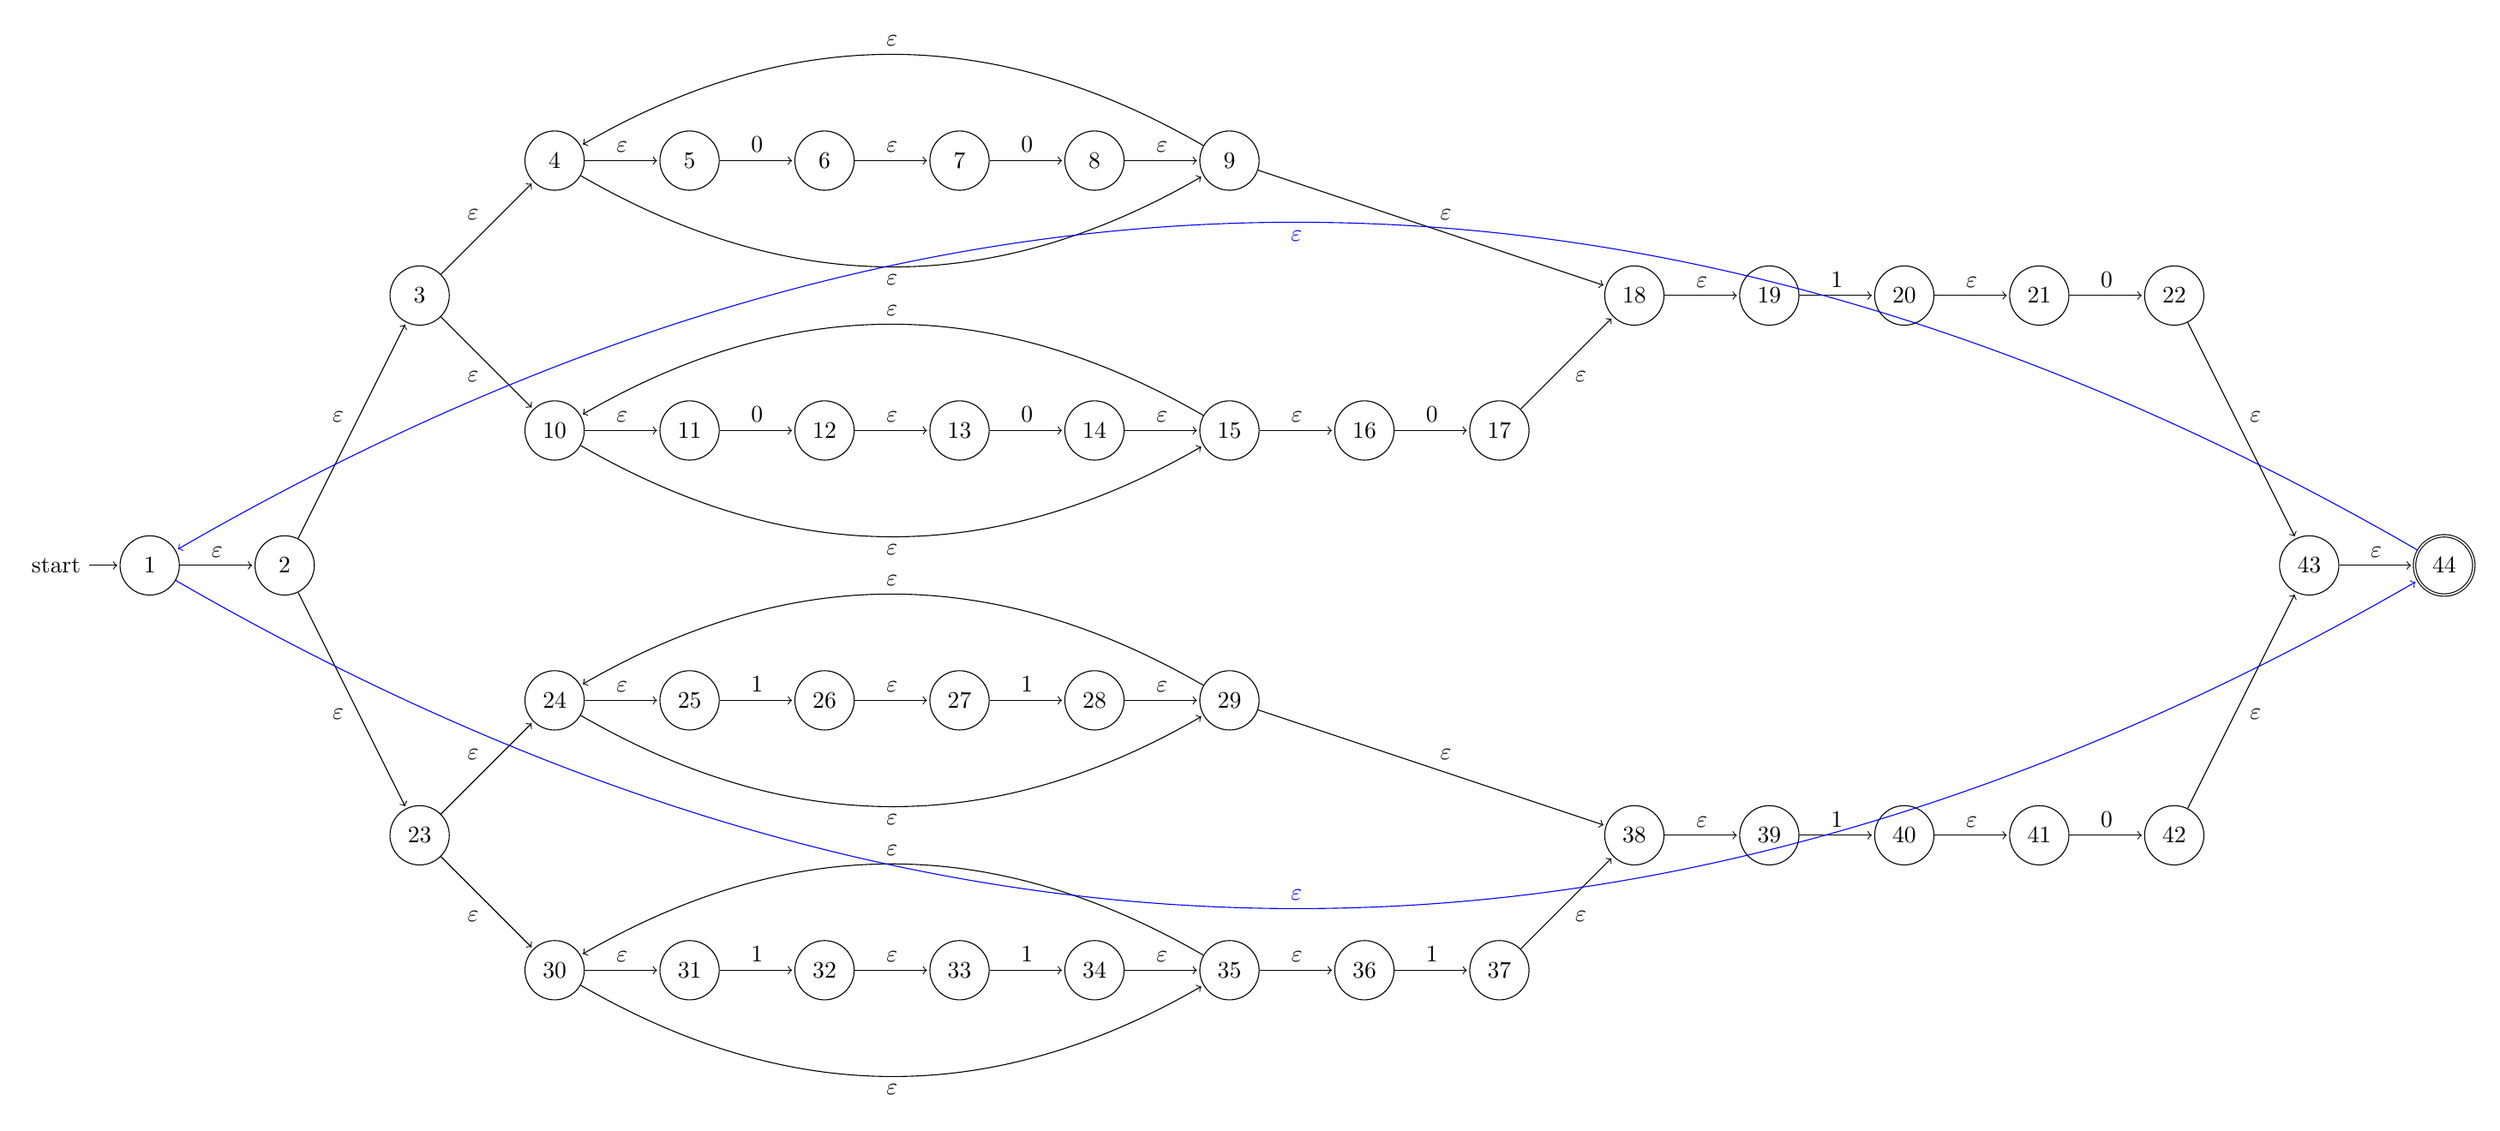
\begin{tikzpicture}[shorten >=1pt,node distance=2cm,auto]
        \tikzstyle{invisible}=[draw=white]

        \node[state,invisible]  (I01)             { }; % E7
        \node[state]  (Q03) [left of=I01]         {3};
        \node[state]  (Q04) [above of=I01]        {4};
        \node[state]  (Q05) [right of=Q04]        {5};
        \node[state]  (Q06) [right of=Q05]        {6};
        \node[state]  (Q07) [right of=Q06]        {7};
        \node[state]  (Q08) [right of=Q07]        {8};
        \node[state]  (Q09) [right of=Q08]        {9};
        \node[state]  (Q10) [below of=I01]        {10};
        \node[state]  (Q11) [right of=Q10]        {11};
        \node[state]  (Q12) [right of=Q11]        {12};
        \node[state]  (Q13) [right of=Q12]        {13};
        \node[state]  (Q14) [right of=Q13]        {14};
        \node[state]  (Q15) [right of=Q14]        {15};
        \node[state]  (Q16) [right of=Q15]        {16};
        \node[state]  (Q17) [right of=Q16]        {17};
        \node[state,invisible]  (I02) [above of=Q17] { };
        \node[state]  (Q18) [right of=I02]        {18};
        \node[state]  (Q19) [right of=Q18]        {19};
        \node[state]  (Q20) [right of=Q19]        {20};
        \node[state]  (Q21) [right of=Q20]        {21};
        \node[state]  (Q22) [right of=Q21]        {22};

        \node[state,invisible]  (I05) [below of=Q03] { };
        \node[state,invisible]  (I06) [below of=I05] { };
        \node[state,invisible]  (I07) [below of=I06] { };
        \node[state]  (Q02) [left of=I06]        {2};

        \node[state]  (Q23) [below of=I07]        {23};
        \node[state,invisible]  (I03) [right of=Q23] { }; % E8
        \node[state]  (Q24) [above of=I03]        {24};
        \node[state]  (Q25) [right of=Q24]        {25};
        \node[state]  (Q26) [right of=Q25]        {26};
        \node[state]  (Q27) [right of=Q26]        {27};
        \node[state]  (Q28) [right of=Q27]        {28};
        \node[state]  (Q29) [right of=Q28]        {29};
        \node[state]  (Q30) [below of=I03]        {30};
        \node[state]  (Q31) [right of=Q30]        {31};
        \node[state]  (Q32) [right of=Q31]        {32};
        \node[state]  (Q33) [right of=Q32]        {33};
        \node[state]  (Q34) [right of=Q33]        {34};
        \node[state]  (Q35) [right of=Q34]        {35};
        \node[state]  (Q36) [right of=Q35]        {36};
        \node[state]  (Q37) [right of=Q36]        {37};
        \node[state,invisible]  (I04) [above of=Q37] { };
        \node[state]  (Q38) [right of=I04]        {38};
        \node[state]  (Q39) [right of=Q38]        {39};
        \node[state]  (Q40) [right of=Q39]        {40};
        \node[state]  (Q41) [right of=Q40]        {41};
        \node[state]  (Q42) [right of=Q41]        {42};

        \node[state,invisible]  (I08) [below of=Q22] { };
        \node[state,invisible]  (I09) [below of=I08] { };
        \node[state]  (Q43) [right of=I09] {43};

        \node[state,accepting]  (Q44) [right of=Q43] {44};
        \node[state,initial]  (Q01) [left of=Q02] {1};

        \path[->]
                  (Q02) edge node                     {$\varepsilon$} (Q03)
                        edge node [swap]              {$\varepsilon$} (Q23)
                  (Q01) edge node                     {$\varepsilon$} (Q02)
                  (Q04) edge node                     {$\varepsilon$} (Q05)% E7
                        edge [bend right] node [swap] {$\varepsilon$} (Q09)
                  (Q05) edge node                     {0}             (Q06)
                  (Q06) edge node                     {$\varepsilon$} (Q07)
                  (Q07) edge node                     {0}             (Q08)
                  (Q08) edge node                     {$\varepsilon$} (Q09)
                  (Q09) edge [bend right] node [swap] {$\varepsilon$} (Q04)
                  (Q09) edge node                     {$\varepsilon$} (Q18)
                  (Q10) edge node                     {$\varepsilon$} (Q11)
                        edge [bend right] node [swap] {$\varepsilon$} (Q15)
                  (Q11) edge node                     {0}             (Q12)
                  (Q12) edge node                     {$\varepsilon$} (Q13)
                  (Q13) edge node                     {0}             (Q14)
                  (Q14) edge node                     {$\varepsilon$} (Q15)
                  (Q15) edge [bend right] node [swap] {$\varepsilon$} (Q10)
                        edge node                     {$\varepsilon$} (Q16)
                  (Q16) edge node                     {0}             (Q17)
                  (Q17) edge node [swap]              {$\varepsilon$} (Q18)
                  (Q03) edge node                     {$\varepsilon$} (Q04)
                        edge node [swap]              {$\varepsilon$} (Q10)
                  (Q18) edge node                     {$\varepsilon$} (Q19)
                  (Q19) edge node                     {1}             (Q20)
                  (Q20) edge node                     {$\varepsilon$} (Q21)
                  (Q21) edge node                     {0}             (Q22)
                  (Q22) edge node                     {$\varepsilon$} (Q43)

                  (Q24) edge node                     {$\varepsilon$} (Q25)% E8
                        edge [bend right] node [swap] {$\varepsilon$} (Q29)
                  (Q25) edge node                     {1}             (Q26)
                  (Q26) edge node                     {$\varepsilon$} (Q27)
                  (Q27) edge node                     {1}             (Q28)
                  (Q28) edge node                     {$\varepsilon$} (Q29)
                  (Q29) edge [bend right] node [swap] {$\varepsilon$} (Q24)
                  (Q29) edge node                     {$\varepsilon$} (Q38)
                  (Q30) edge node                     {$\varepsilon$} (Q31)
                        edge [bend right] node [swap] {$\varepsilon$} (Q35)
                  (Q31) edge node                     {1}             (Q32)
                  (Q32) edge node                     {$\varepsilon$} (Q33)
                  (Q33) edge node                     {1}             (Q34)
                  (Q34) edge node                     {$\varepsilon$} (Q35)
                  (Q35) edge [bend right] node [swap] {$\varepsilon$} (Q30)
                        edge node                     {$\varepsilon$} (Q36)
                  (Q36) edge node                     {1}             (Q37)
                  (Q37) edge node [swap]              {$\varepsilon$} (Q38)
                  (Q23) edge node                     {$\varepsilon$} (Q24)
                        edge node [swap]              {$\varepsilon$} (Q30)
                  (Q38) edge node                     {$\varepsilon$} (Q39)
                  (Q39) edge node                     {1}             (Q40)
                  (Q40) edge node                     {$\varepsilon$} (Q41)
                  (Q41) edge node                     {0}             (Q42)
                  (Q42) edge node [swap]              {$\varepsilon$} (Q43)
                  (Q43) edge node                     {$\varepsilon$} (Q44);
        \path[->][blue]
                  (Q01) edge [bend right] node        {$\varepsilon$} (Q44)
                  (Q44) edge [bend right] node        {$\varepsilon$} (Q01);
      \end{tikzpicture}
      \end{adjustbox}
      \end{center}

    \end{itemize}

    \newpage
    \item Generate the equivalent $DFA$ \\ \\
          To generate the equivalent DFA, we'll follow the \textbf{subset construction method},
so we'll need the equivalent NFA. In the table \ref{tab:ENFA}(a) we have the transition
table of \ENFA and in the table \ref{tab:ENFA}(b) the closures.

\begin{table}[h]
  \centering
  \caption{Transition Table of \ENFA}
  \label{tab:ENFA}
  \subfloat[{\tiny Transition Table of {\normalsize $\varepsilon$}$-NFA$}]{
    \hspace{.2cm}
    \scalebox{0.7}{ \begin{tabular}[c]{|c|c|c|c|} \hline
  States & 0 & 1 & $\varepsilon$ \\ \hline
     1 & & & 2 44 \\ \hline
     2 & & & 3 23 \\ \hline
     3 & & & 4 10 \\ \hline
     4 & & & 5 9 \\ \hline
     5 & 6 & & \\ \hline
     6 & & & 7 \\ \hline
     7 & 8 & & \\ \hline
     8 & & & 9 \\ \hline
     9 & & & 4 18 \\ \hline
    10 & & & 11 15\\ \hline
    11 & 12 & & \\ \hline
    12 & & & 13 \\ \hline
    13 & 14 & & \\ \hline
    14 & & & 15 \\ \hline
    15 & & & 10 16\\ \hline
    16 & 17 & & \\ \hline
    17 & & & 18\\ \hline
    18 & & & 19\\ \hline
    19 & & 20 & \\ \hline
    20 & & & 21 \\ \hline
    21 & 22 & & \\ \hline
    22 & & & 43 \\ \hline
    23 & & & 24 30 \\ \hline
    24 & & & 25 29 \\ \hline
    25 & & 26 & \\ \hline
    26 & & & 27 \\ \hline
    27 & & 28 & \\ \hline
    28 & & & 29 \\ \hline
    29 & & & 24 38 \\ \hline
    30 & & & 31 35 \\ \hline
    31 & & 32 & \\ \hline
    32 & & & 33 \\ \hline
    33 & & 34 & \\ \hline
    34 & & & 35 \\ \hline
    35 & & & 30 36 \\ \hline
    36 & & 37 & \\ \hline
    37 & & & 38 \\ \hline
    38 & & & 39 \\ \hline
    39 & & 40 & \\ \hline
    40 & & & 41 \\ \hline
    41 & 42 & & \\ \hline
    42 & & & 43 \\ \hline
    43 & & & 44 \\ \hline
    44 & & & 1 \\ \hline
\end{tabular}
 }
    \hspace{.2cm}
  }
  \hspace{1cm}
  \subfloat[{\tiny Closures of {\normalsize $\varepsilon$}$-NFA$}]{
    \hspace{.2cm}
    \scalebox{0.7}{ \begin{tabular}[c]{r|c|c|} \cline{2-3}
    & States & Closures \\ \cline{2-3}
    $\rightarrow *$ & 1 & 1 2 44 3 23 4 10 24 30 5 9 18 19 11 15 25 29 31 35 16 38 36 39 \\ \cline{2-3}
    & 2 & 2 3 23 4 10 24 30 5 9 11 15 25 29 31 35 18 16 38 36 19 39 \\ \cline{2-3}
    & 3 & 3 4 10 5 9 11 15 18 16 19 \\ \cline{2-3}
    & 4 & 4 5 9 18 19 \\ \cline{2-3}
    & 5 & 5 \\ \cline{2-3}
    & 6 & 6 7 \\ \cline{2-3}
    & 7 & 7 \\ \cline{2-3}
    & 8 & 8 9 4 18 5 19 \\ \cline{2-3}
    & 9 & 9 4 18 5 19 \\ \cline{2-3}
    & 10 & 10 11 15 16 \\ \cline{2-3}
    & 11 & 11 \\ \cline{2-3}
    & 12 & 12 13 \\ \cline{2-3}
    & 13 & 13 \\ \cline{2-3}
    & 14 & 14 15 10 16 11 \\ \cline{2-3}
    & 15 & 15 10 16 11 \\ \cline{2-3}
    & 16 & 16 \\ \cline{2-3}
    & 17 & 17 18 19 \\ \cline{2-3}
    & 18 & 18 19 \\ \cline{2-3}
    & 19 & 19 \\ \cline{2-3}
    & 20 & 20 21 \\ \cline{2-3}
    & 21 & 21 \\ \cline{2-3}
    $*$ & 22 & 22 43 44 1 2 3 23 4 10 24 30 5 9 18 19 11 15 25 29 31 35 16 38 36 39 \\ \cline{2-3}
    & 23 & 23 24 25 29 38 39 30 31 35 36 \\ \cline{2-3}
    & 24 & 24 25 29 38 39 \\ \cline{2-3}
    & 25 & 25 \\ \cline{2-3}
    & 26 & 26 27 \\ \cline{2-3}
    & 27 & 27 \\ \cline{2-3}
    & 28 & 28 29 24 38 25 39 \\ \cline{2-3}
    & 29 & 29 24 38 25 39 \\ \cline{2-3}
    & 30 & 30 31 35 36 \\ \cline{2-3}
    & 31 & 31 \\ \cline{2-3}
    & 32 & 32 33 \\ \cline{2-3}
    & 33 & 33 \\ \cline{2-3}
    & 34 & 34 35 30 36 31 \\ \cline{2-3}
    & 35 & 35 30 36 31 \\ \cline{2-3}
    & 36 & 36 \\ \cline{2-3}
    & 37 & 37 38 39 \\ \cline{2-3}
    & 38 & 38 39 \\ \cline{2-3}
    & 39 & 39 \\ \cline{2-3}
    & 40 & 40 41 \\ \cline{2-3}
    & 41 & 41 \\ \cline{2-3}
    $*$ & 42 & 42 43 44 1 2 3 23 4 10 24 30 5 9 18 19 11 15 25 29 31 35 16 38 36 39 \\ \cline{2-3}
    $*$ & 43 & 43 44 1 2 3 23 4 10 24 30 5 9 18 19 11 15 25 29 31 35 16 38 36 39 \\ \cline{2-3}
    $*$ & 44 & 44 1 2 3 23 4 10 24 30 5 9 18 19 11 15 25 29 31 35 16 38 36 39 \\ \cline{2-3}
\end{tabular}
 }
    \hspace{.2cm}
  }
\end{table}

\newpage
Removing the {\Large $\varepsilon$}-transition, we obtain the transition
table \ref{tab:NFA} of NFA.

\begin{table}[h!]
\centering
  \scalebox{0.6}{ \begin{tabular}[c]{r|c|c|c|} \cline{2-4}
    & States & 0 & 1 \\ \cline{2-4}
    $\rightarrow *$ & 1 & 6 12 17 & 20 26 32 37 40 \\ \cline{2-4}
    & 2 & 6 12 17 & 20 26 32 37 40 \\ \cline{2-4}
    & 3 & 6 12 17 & 20 \\ \cline{2-4}
    & 4 & 6 & 20 \\ \cline{2-4}
    & 5 & 6 & \\ \cline{2-4}
    & 6 & 8 & \\ \cline{2-4}
    & 7 & 8 & \\ \cline{2-4}
    & 8 & 6 & 20 \\ \cline{2-4}
    & 9 & 6 & 20 \\ \cline{2-4}
    & 10 & 12 17 & \\ \cline{2-4}
    & 11 & 12 & \\ \cline{2-4}
    & 12 & 14 & \\ \cline{2-4}
    & 13 & 14 & \\ \cline{2-4}
    & 14 & 12 17 & \\ \cline{2-4}
    & 15 & 12 17 & \\ \cline{2-4}
    & 16 & 17 & \\ \cline{2-4}
    & 17 & & 20 \\ \cline{2-4}
    & 18 & & 20 \\ \cline{2-4}
    & 19 & & 20 \\ \cline{2-4}
    & 20 & 22 & \\ \cline{2-4}
    & 21 & 22 & \\ \cline{2-4}
    $*$ & 22 & 6 12 17 & 20 26 32 37 40 \\ \cline{2-4}
    & 23 & & 26 32 37 40 \\ \cline{2-4}
    & 24 & & 26 40 \\ \cline{2-4}
    & 25 & & 26 \\ \cline{2-4}
    & 26 & & 28 \\ \cline{2-4}
    & 27 & & 28 \\ \cline{2-4}
    & 28 & & 26 40 \\ \cline{2-4}
    & 29 & & 26 40 \\ \cline{2-4}
    & 30 & & 32 37 \\ \cline{2-4}
    & 31 & & 32 \\ \cline{2-4}
    & 32 & & 34 \\ \cline{2-4}
    & 33 & & 34 \\ \cline{2-4}
    & 34 & & 32 37 \\ \cline{2-4}
    & 35 & & 32 37 \\ \cline{2-4}
    & 36 & & 37 \\ \cline{2-4}
    & 37 & & 40 \\ \cline{2-4}
    & 38 & & 40 \\ \cline{2-4}
    & 39 & & 40 \\ \cline{2-4}
    & 40 & 42 & \\ \cline{2-4}
    & 41 & 42 & \\ \cline{2-4}
    $*$ & 42 & 6 12 17 & 20 26 32 37 40 \\ \cline{2-4}
    $*$ & 43 & 6 12 17 & 20 26 32 37 40 \\ \cline{2-4}
    $*$ & 44 & 6 12 17 & 20 26 32 37 40 \\ \cline{2-4}
\end{tabular}
 }
  \caption{Transition Table of NFA}
  \label{tab:NFA}
\end{table}

And the NFA: \\
\begin{center}
\begin{adjustbox}{max width=14cm}
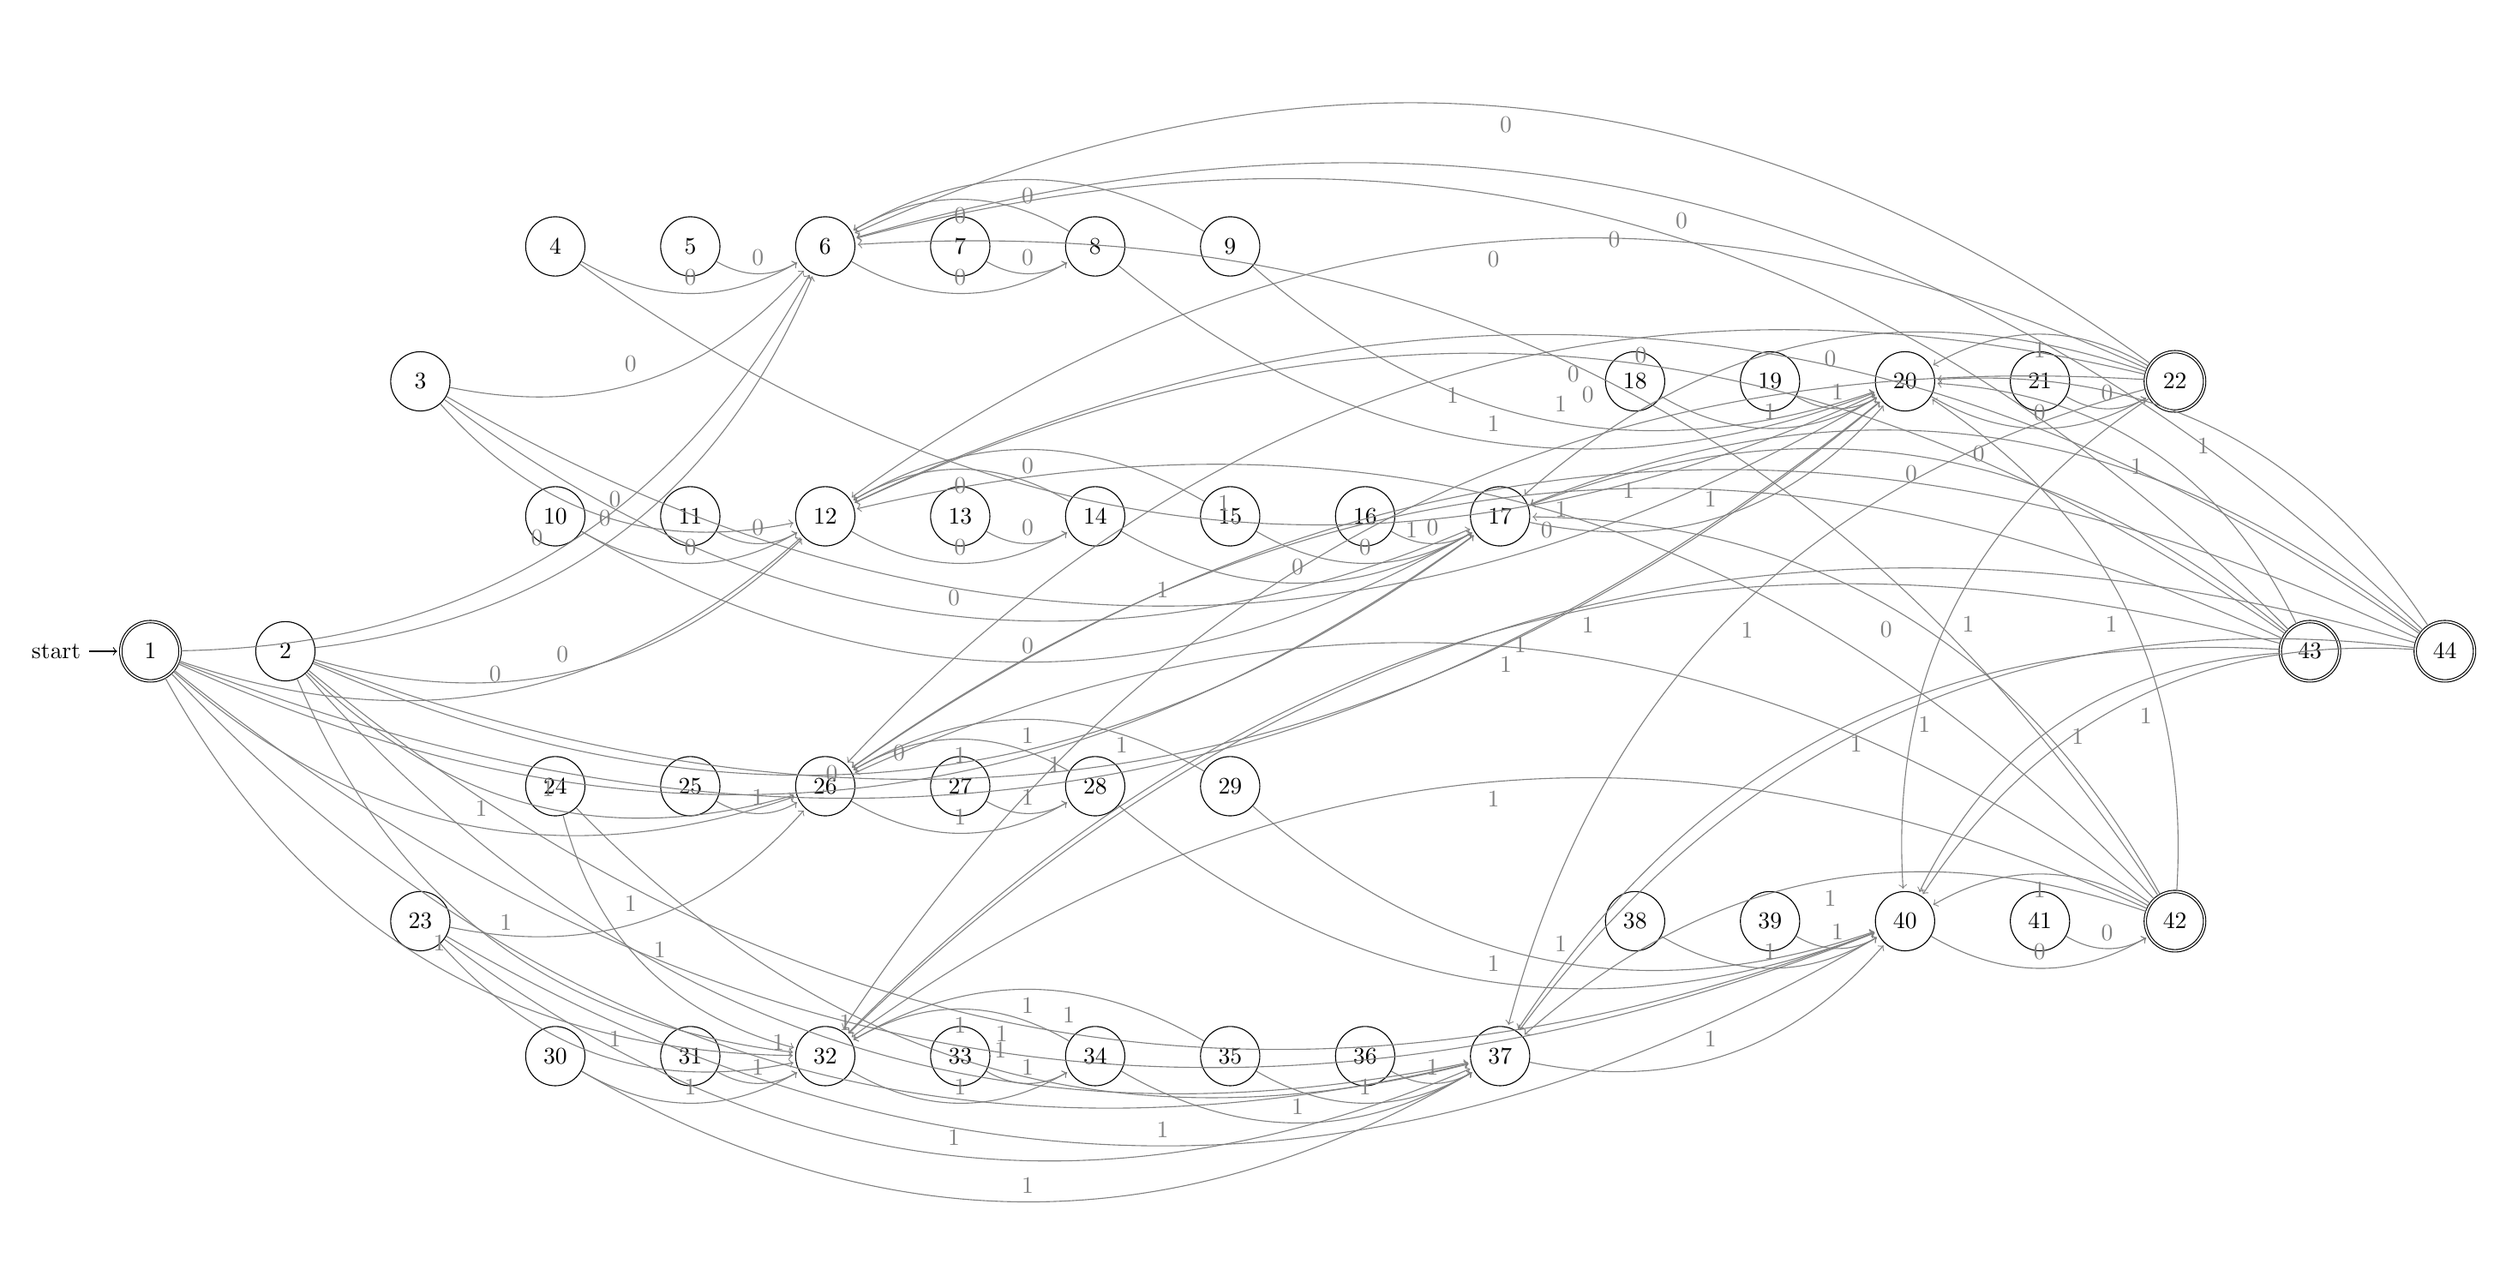
\begin{tikzpicture}[shorten >=1pt,node distance=2cm,auto]
  \tikzstyle{invisible}=[draw=white]

  \node[state,invisible]  (I01)             { };
  \node[state]  (Q03) [left of=I01]         {3};
  \node[state]  (Q04) [above of=I01]        {4};
  \node[state]  (Q05) [right of=Q04]        {5};
  \node[state]  (Q06) [right of=Q05]        {6};
  \node[state]  (Q07) [right of=Q06]        {7};
  \node[state]  (Q08) [right of=Q07]        {8};
  \node[state]  (Q09) [right of=Q08]        {9};
  \node[state]  (Q10) [below of=I01]        {10};
  \node[state]  (Q11) [right of=Q10]        {11};
  \node[state]  (Q12) [right of=Q11]        {12};
  \node[state]  (Q13) [right of=Q12]        {13};
  \node[state]  (Q14) [right of=Q13]        {14};
  \node[state]  (Q15) [right of=Q14]        {15};
  \node[state]  (Q16) [right of=Q15]        {16};
  \node[state]  (Q17) [right of=Q16]        {17};
  \node[state,invisible]  (I02) [above of=Q17] { };
  \node[state]  (Q18) [right of=I02]        {18};
  \node[state]  (Q19) [right of=Q18]        {19};
  \node[state]  (Q20) [right of=Q19]        {20};
  \node[state]  (Q21) [right of=Q20]        {21};
  \node[state,accepting]  (Q22) [right of=Q21]        {22};

  \node[state,invisible]  (I05) [below of=Q03] { };
  \node[state,invisible]  (I06) [below of=I05] { };
  \node[state,invisible]  (I07) [below of=I06] { };
  \node[state]  (Q02) [left of=I06]        {2};

  \node[state]  (Q23) [below of=I07]        {23};
  \node[state,invisible]  (I03) [right of=Q23] { };
  \node[state]  (Q24) [above of=I03]        {24};
  \node[state]  (Q25) [right of=Q24]        {25};
  \node[state]  (Q26) [right of=Q25]        {26};
  \node[state]  (Q27) [right of=Q26]        {27};
  \node[state]  (Q28) [right of=Q27]        {28};
  \node[state]  (Q29) [right of=Q28]        {29};
  \node[state]  (Q30) [below of=I03]        {30};
  \node[state]  (Q31) [right of=Q30]        {31};
  \node[state]  (Q32) [right of=Q31]        {32};
  \node[state]  (Q33) [right of=Q32]        {33};
  \node[state]  (Q34) [right of=Q33]        {34};
  \node[state]  (Q35) [right of=Q34]        {35};
  \node[state]  (Q36) [right of=Q35]        {36};
  \node[state]  (Q37) [right of=Q36]        {37};
  \node[state,invisible]  (I04) [above of=Q37] { };
  \node[state]  (Q38) [right of=I04]        {38};
  \node[state]  (Q39) [right of=Q38]        {39};
  \node[state]  (Q40) [right of=Q39]        {40};
  \node[state]  (Q41) [right of=Q40]        {41};
  \node[state,accepting]  (Q42) [right of=Q41]        {42};

  \node[state,invisible]  (I08) [below of=Q22] { };
  \node[state,invisible]  (I09) [below of=I08] { };
  \node[state,accepting]  (Q43) [right of=I09] {43};

  \node[state,accepting]  (Q44) [right of=Q43] {44};
  \node[state,initial,accepting]  (Q01) [left of=Q02] {1};

  \path[->][gray]
            (Q01) edge [bend right] node {0} (Q06)
                  edge [bend right] node {0} (Q12)
                  edge [bend right] node {0} (Q17)
                  edge [bend right] node {1} (Q20)
                  edge [bend right] node {1} (Q26)
                  edge [bend right] node {1} (Q32)
                  edge [bend right] node {1} (Q37)
                  edge [bend right] node {1} (Q40)
            (Q02) edge [bend right] node {0} (Q06)
                  edge [bend right] node {0} (Q12)
                  edge [bend right] node {0} (Q17)
                  edge [bend right] node {1} (Q20)
                  edge [bend right] node {1} (Q26)
                  edge [bend right] node {1} (Q32)
                  edge [bend right] node {1} (Q37)
                  edge [bend right] node {1} (Q40)
            (Q03) edge [bend right] node {0} (Q06)
                  edge [bend right] node {0} (Q12)
                  edge [bend right] node {0} (Q17)
                  edge [bend right] node {1} (Q20)
            (Q04) edge [bend right] node {0} (Q06)
                  edge [bend right] node {1} (Q20)
            (Q05) edge [bend right] node {0} (Q06)
            (Q06) edge [bend right] node {0} (Q08)
            (Q07) edge [bend right] node {0} (Q08)
            (Q08) edge [bend right] node {0} (Q06)
                  edge [bend right] node {1} (Q20)
            (Q09) edge [bend right] node {0} (Q06)
                  edge [bend right] node {1} (Q20)
            (Q10) edge [bend right] node {0} (Q12)
                  edge [bend right] node {0} (Q17)
            (Q11) edge [bend right] node {0} (Q12)
            (Q12) edge [bend right] node {0} (Q14)
            (Q13) edge [bend right] node {0} (Q14)
            (Q14) edge [bend right] node {0} (Q12)
                  edge [bend right] node {0} (Q17)
            (Q15) edge [bend right] node {0} (Q12)
                  edge [bend right] node {0} (Q17)
            (Q16) edge [bend right] node {0} (Q17)
            (Q17) edge [bend right] node {1} (Q20)
            (Q18) edge [bend right] node {1} (Q20)
            (Q19) edge [bend right] node {1} (Q20)
            (Q20) edge [bend right] node {0} (Q22)
            (Q21) edge [bend right] node {0} (Q22)
            (Q22) edge [bend right] node {0} (Q06)
                  edge [bend right] node {0} (Q12)
                  edge [bend right] node {0} (Q17)
                  edge [bend right] node {1} (Q20)
                  edge [bend right] node {1} (Q26)
                  edge [bend right] node {1} (Q32)
                  edge [bend right] node {1} (Q37)
                  edge [bend right] node {1} (Q40)
            (Q23) edge [bend right] node {1} (Q26)
                  edge [bend right] node {1} (Q32)
                  edge [bend right] node {1} (Q37)
                  edge [bend right] node {1} (Q40)
            (Q24) edge [bend right] node {1} (Q32)
                  edge [bend right] node {1} (Q37)
            (Q25) edge [bend right] node {1} (Q26)
            (Q26) edge [bend right] node {1} (Q28)
            (Q27) edge [bend right] node {1} (Q28)
            (Q28) edge [bend right] node {1} (Q26)
                  edge [bend right] node {1} (Q40)
            (Q29) edge [bend right] node {1} (Q26)
                  edge [bend right] node {1} (Q40)
            (Q30) edge [bend right] node {1} (Q32)
                  edge [bend right] node {1} (Q37)
            (Q31) edge [bend right] node {1} (Q32)
            (Q32) edge [bend right] node {1} (Q34)
            (Q33) edge [bend right] node {1} (Q34)
            (Q34) edge [bend right] node {1} (Q32)
                  edge [bend right] node {1} (Q37)
            (Q35) edge [bend right] node {1} (Q32)
                  edge [bend right] node {1} (Q37)
            (Q36) edge [bend right] node {1} (Q37)
            (Q37) edge [bend right] node {1} (Q40)
            (Q38) edge [bend right] node {1} (Q40)
            (Q39) edge [bend right] node {1} (Q40)
            (Q40) edge [bend right] node {0} (Q42)
            (Q41) edge [bend right] node {0} (Q42)
            (Q42) edge [bend right] node {0} (Q06)
                  edge [bend right] node {0} (Q12)
                  edge [bend right] node {0} (Q17)
                  edge [bend right] node {1} (Q20)
                  edge [bend right] node {1} (Q26)
                  edge [bend right] node {1} (Q32)
                  edge [bend right] node {1} (Q37)
                  edge [bend right] node {1} (Q40)
            (Q43) edge [bend right] node {0} (Q06)
                  edge [bend right] node {0} (Q12)
                  edge [bend right] node {0} (Q17)
                  edge [bend right] node {1} (Q20)
                  edge [bend right] node {1} (Q26)
                  edge [bend right] node {1} (Q32)
                  edge [bend right] node {1} (Q37)
                  edge [bend right] node {1} (Q40)
            (Q44) edge [bend right] node {0} (Q06)
                  edge [bend right] node {0} (Q12)
                  edge [bend right] node {0} (Q17)
                  edge [bend right] node {1} (Q20)
                  edge [bend right] node {1} (Q26)
                  edge [bend right] node {1} (Q32)
                  edge [bend right] node {1} (Q37)
                  edge [bend right] node {1} (Q40);

\end{tikzpicture}
\end{adjustbox}
\end{center}


\newpage
Following the \textbf{subset construction method}, we obtain the table
\refeq{tab:DFA}(a) and we can rename the states like in the table \ref{tab:DFA}(b).

\begin{table}[h]
  \centering
  \caption{Transition Table of DFA}
  \label{tab:DFA}
  \subfloat[{\tiny Transition Table of DFA}]{
    \hspace{.2cm}
    \scalebox{0.7}{ \begin{tabular}[c]{r|c|c|c|} \cline{2-4}
    & States & 0 & 1 \\ \cline{2-4}
    $\rightarrow *$ A & 1 & 6\_12\_17 & 20\_26\_32\_37\_40 \\ \cline{2-4}
    B & 6\_12\_17 & 8\_14 & 20  \\ \cline{2-4}
    C & 20\_26\_32\_37\_40 & 22\_42 & 28\_34\_40 \\ \cline{2-4}
    D & 8\_14 & 6\_12\_17 & 20 \\ \cline{2-4}
    E & 20 & 22 & Dead \\ \cline{2-4}
    $*$ F & 22\_42 & 6\_12\_17 & 20\_26\_32\_37\_40 \\ \cline{2-4}
    G & 28\_34\_40 & 42 & 26\_40\_32\_37 \\ \cline{2-4}
    $*$ H & 22 & 6\_12\_17 & 20\_26\_32\_37\_40 \\ \cline{2-4}
    $*$ I & 42 & 6\_12\_17 & 20\_26\_32\_37\_40 \\ \cline{2-4}
    J & 26\_40\_32\_37 & 42 & 28\_34\_40 \\ \cline{2-4}
    & Dead & Dead & Dead \\ \cline{2-4}
\end{tabular}
 }
    \hspace{.2cm}
  }
  \hspace{1cm}
  \subfloat[{\tiny Transition Table of DFA (Renamed)}]{
    \hspace{.2cm}
    \scalebox{0.7}{ \begin{tabular}[c]{r|c|c|c|} \cline{2-4}
    & States & 0 & 1 \\ \cline{2-4}
    $\rightarrow *$ & A & B & C \\ \cline{2-4}
    & B & D & E  \\ \cline{2-4}
    & C & F & G \\ \cline{2-4}
    & D & B & E \\ \cline{2-4}
    & E & H & Dead \\ \cline{2-4}
    $*$ & F & B & C \\ \cline{2-4}
    & G & I & J \\ \cline{2-4}
    $*$ & H & B & C \\ \cline{2-4}
    $*$ & I & B & C \\ \cline{2-4}
    & J & I & G \\ \cline{2-4}
    & Dead & Dead & Dead \\ \cline{2-4}
\end{tabular}
 }
    \hspace{.2cm}
  }
\end{table}

Following the \textbf{state minimization algorithm} for DFAs, we obtain the table \ref{tab:MinztDFA}
where {\small\textcolor{red}{X}} are all initial pairs of distinguishable states,
{\small\textcolor{blue}{X}} are all pairs of distinguishable states in the first round and
{\small\textcolor{gray}{O}} are all pairs of equivalent states.
\begin{table}[h!]
\centering
  \scalebox{0.9}{ \begin{tabular}[c]{rccccccccccc}

                  &      &   &   &   &   &   &   &   &   &   & $\rightarrow$ \\
                  &      &   &$*$&$*$&   &$*$&   &   &   &   & $*$ \\
                  &      & J & I & H & G & F & E & D & C & B & A \\
                  & Dead & \textcolor{blue}{X} & \textcolor{red}{X} & \textcolor{red}{X} & \textcolor{blue}{X} & \textcolor{red}{X} & \textcolor{blue}{X} & \textcolor{blue}{X} & \textcolor{blue}{X} & \textcolor{blue}{X} & \textcolor{red}{X} \\
  $\rightarrow*$  & A    & \textcolor{red}{X} & \textcolor{gray}{O} & \textcolor{gray}{O} & \textcolor{red}{X} & \textcolor{gray}{O} & \textcolor{red}{X} & \textcolor{red}{X} & \textcolor{red}{X} & \textcolor{red}{X} &   \\
                  & B    & \textcolor{blue}{X} & \textcolor{red}{X} & \textcolor{red}{X} & \textcolor{blue}{X} & \textcolor{red}{X} & \textcolor{blue}{X} & \textcolor{gray}{O} & \textcolor{blue}{X} &   &   \\
                  & C    & \textcolor{gray}{O} & \textcolor{red}{X} & \textcolor{red}{X} & \textcolor{gray}{O} & \textcolor{red}{X} & \textcolor{blue}{X} & \textcolor{blue}{X} &   &   &   \\
                  & D    & \textcolor{blue}{X} & \textcolor{red}{X} & \textcolor{red}{X} & \textcolor{blue}{X} & \textcolor{red}{X} & \textcolor{blue}{X} &   &   &   &   \\
                  & E    & \textcolor{blue}{X} & \textcolor{red}{X} & \textcolor{red}{X} & \textcolor{blue}{X} & \textcolor{red}{X} &   &   &   &   &   \\
             $*$  & F    & \textcolor{red}{X} & \textcolor{gray}{O} & \textcolor{gray}{O} & \textcolor{red}{X} &   &   &   &   &   &   \\
                  & G    & \textcolor{gray}{O} & \textcolor{red}{X} & \textcolor{red}{X} &   &   &   &   &   &   &   \\
             $*$  & H    & \textcolor{red}{X} & \textcolor{gray}{O} &   &   &   &   &   &   &   &   \\
             $*$  & I    & \textcolor{red}{X} &   &   &   &   &   &   &   &   &   \\
\end{tabular}
 }
  \caption{Minimization Table of DFA}
  \label{tab:MinztDFA}
\end{table}

\newpage

The Minimum-state DFA is:
\begin{table}[h]
  \centering
  \caption{Minimum-state Table of DFA}
  \label{tab:MinDFA}
  \subfloat[{\tiny Minimum-state Table of DFA}]{
    \hspace{.2cm}
    \scalebox{1}{ \begin{tabular}[c]{r|c|c|c|} \cline{2-4}
    & States & 0 & 1 \\ \cline{2-4}
    $\rightarrow *$ & A\_I\_H\_F & B\_D & C\_J\_G \\ \cline{2-4}
    & B\_D & B\_D & E \\ \cline{2-4}
    & E & A\_I\_H\_F & Dead \\ \cline{2-4}
    & C\_J\_G & A\_I\_H\_F & C\_J\_G \\ \cline{2-4}
    & Dead & Dead & Dead \\ \cline{2-4}

\end{tabular}
 }
    \hspace{.2cm}
  }
  \hspace{1cm}
  \subfloat[{\tiny Minimum-state Table of DFA (Renamed)}]{
    \hspace{.2cm}
    \scalebox{1}{ \begin{tabular}[c]{r|c|c|c|} \cline{2-4}
    & States & 0 & 1 \\ \cline{2-4}
    $\rightarrow *$ & A & B & C \\ \cline{2-4}
    & B & B & D \\ \cline{2-4}
    & D & A & Dead \\ \cline{2-4}
    & C & A & C \\ \cline{2-4}
    & Dead & Dead & Dead \\ \cline{2-4}

\end{tabular}
 }
    \hspace{.2cm}
  }
\end{table}

\begin{center}
\begin{adjustbox}{max width=14cm}
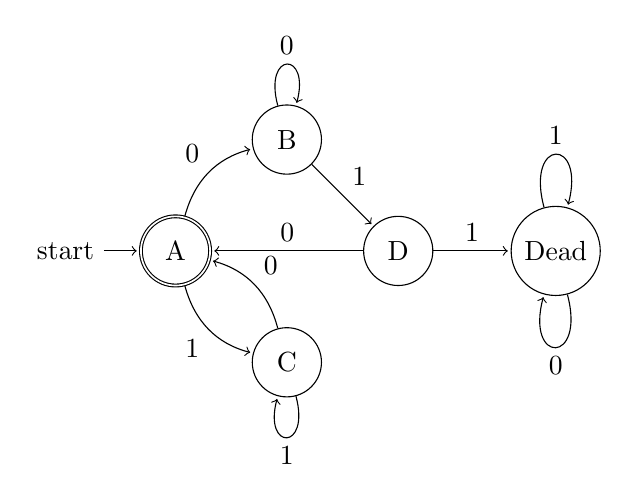
\begin{tikzpicture}[shorten >=1pt,node distance=2cm,auto]

  \node[state,initial,accepting]  (A)                         {A};
  \node[state]                    (B)     [above right of=A]  {B};
  \node[state]                    (C)     [below right of=A]  {C};
  \node[state]                    (D)     [below right of=B]  {D};
  \node[state]                    (Dead)  [right of=D]        {Dead};

  \path[->]
            (A) edge [bend left]  node {0} (B)
                edge [bend right] node [swap] {1} (C)
            (B) edge [loop above] node {0} ()
                edge              node {1} (D)
            (C) edge [loop below] node {1} ()
                edge [bend right] node [swap] {0} (A)
            (D) edge              node [swap] {0} (A)
                edge              node {1} (Dead)
            (Dead) edge [loop above] node {1} ()
                   edge [loop below] node {0} ();
\end{tikzpicture}
\end{adjustbox}
\end{center}


    \newpage
    \item Implement it in a programming language (\verb!Python!,
          \verb!C!/\verb!C++!, \verb!Java!) following the table method. \\ \\
          Solution 3.


  \end{enumerate}

\end{document}
